% Podstawowe definicje dla wszystkich dokumentów

\documentclass[11pt]{mwart}
%\setlength{\textwidth}{83pt}

\usepackage[OT4,plmath]{polski}
\usepackage{amsmath,amssymb,amsfonts,amsthm,mathtools}
\usepackage{color}
\usepackage{fontspec}
\usepackage{listings,times}

\usepackage{bbm}
\usepackage[colorlinks=true, urlcolor=blue]{hyperref}
\usepackage{url}
\usepackage{graphicx}

\graphicspath{{images/}}

\newcommand{\HRule}{\rule{\linewidth}{0.5mm}}

\newcommand{\term}[1]{
  \indent\textbf{#1}
  \vspace{5pt}
}

\usepackage{multicol}

\usepackage{lmodern} \normalfont
%\DeclareFontShape{EU1}{ptm}{bx}{n} { <-> ssub * cmr/bx/n }{}
%\DeclareFontShape{EU1}{ptm}{m}{sc} { <-> ssub * cmr/m/sc }{}

\usepackage{titletoc}

%\titlecontents{section}[3.8em]{}{\contentslabel{2.3em}}{\hspace*{-2.3em}}{\titlerule*[0.25pc]{ .}\contentspage}{}

\usepackage{fancyhdr}
\pagestyle{fancy}
\lhead[\fancyplain{Projekt Iron Coach - \doctitle}{Projekt Iron Coach - \doctitle}]         
    {\fancyplain{Projekt Iron Coach - \doctitle}{Projekt Iron Coach - \doctitle}}
\lfoot[\fancyplain{Studencka Pracownia Inżynierii Oprogramowania}{Studencka Pracownia Inżynierii Oprogramowania}]                 
    {\fancyplain{Studencka Pracownia Inżynierii Oprogramowania}{Studencka Pracownia Inżynierii Oprogramowania}}
\cfoot[\fancyplain{}{}] {\fancyplain{}{}}
\rfoot[\fancyplain{\thepage} {\thepage}]  {\fancyplain{\thepage}{\thepage}}


%\pagestyle{myheadings}
%\markright{Projekt Iron Coach \hfill \doctitle \hfill \rightmark}


\newcommand{\titlep}[2] {
  \newcommand{\doctitle}{#1}
  \begin{titlepage}
    \begin{center}
      \textsc{\large Studencka Pracownia Inżynierii Oprogramowania}\\
      \textsc{\LARGE Uniwersytet Wrocławski \\Instytut Informatyki}\\[1.5cm]


      \vspace{3cm}

      % Author and supervisor
      \begin{minipage}{\textwidth}
        \begin{center} \Large
          Łukasz \textsc{Czapliński},
          Diana \textsc{Czepirska},
          Artur \textsc{Jarocki}
        \end{center}
      \end{minipage}

      \vspace{0.5cm}



      % Title
      \HRule \\[0.4cm]
      { \Huge \bfseries Iron Coach  \\[1cm] }

      \textsc{\Large #1\\\large Wersja #2}\\[0.5cm]

      \HRule \\[1.5cm]

      \vspace{1cm}

      
\includegraphics[width=0.15\textwidth]{non-starred.png}~\\[1cm]
      
      \vfill
      

      \vspace{1cm}

      % Bottom of the page
      {\large Wrocław 2013}

    \end{center}
  \end{titlepage}
  \clearpage
}

\newcommand{\chist}[1]{
  {\large{Historia zmian}} \\ \vspace{1cm}
  \begin{tabular}{r | l | l}
    Wersja & Opis & Autor \\ 
    \hline
    \noalign{\smallskip}
    #1
  \end{tabular}
}

\begin{document}
\titlep{Prototyp interfejsu na iOS}{1.0}
\chist{1.0 & 20.5-10-26 & Powstanie dokumentu & Łukasz Czapliński\\
        }
\setcounter{tocdepth}{2}
\tableofcontents
\clearpage
\section{Wstęp}
\subsection{Cel dokumentu}
\noindent Ninejszy dokument opisuje makietę interfejsu aplikacji ,,Iron Coach'' w wersji na iOS. Ma ona służyć za podstawę dla gotowej aplikacji. Wymienione zostały problemy, na jakie należy zwrócić uwagę podczas implementacji, razem z sugerowanymi rozwiązaniami. W żadnym wypadku nie jest to kompletna lista i wszystkie aspekty powinny zostać przetestowane.
\subsection{Struktura dokumentu}
\noindent Dokument ten podzielony jest na dwie sekcje: pierwszą z nich stanowi wstęp, natomiast drugą właściwa makieta wraz z opisem. Druga sekcja podzielona jest na podsekcje, z których każda opisuje jeden ekran aplikacji. W każdej podsekcji znajduje się makieta ekranu oraz opis przycisków (wraz z ekranami do których powinny prowadzić). Dodatkowo czasem znajduje się też lista ostrzeżeń -- potencjalnych błędnych danych, jakie może wprowadzić użytkownik na danym ekranie aplikacji.
\section{Makieta}
\subsection{Ekran główny}
\subsubsection{Opis}
\noindent Jest to ekran witający użytkownika po uruchomieniu aplikacji ,,Iron Coach''. Powinien zmieniać się, odzwierciedlając postępy użytkownika: jeśli użytkownik często biega, to powinien znaleźć się tam przycisk od tej właśnie aktywności. Jeśli jest to pierwsze uruchomienie aplikacji, to powinien zachęcić użytkownika do aktywności. Zamieszczono przykładowe makiety dla pierwszego uruchomienia oraz dla użytkownika biegającego często.
\subsubsection{Ekrany}
\begin{minipage}{0.5\textwidth}
  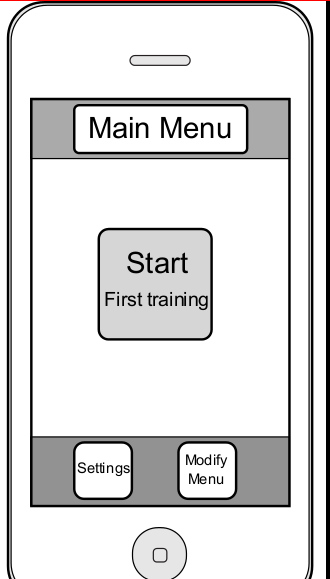
\includegraphics[width=0.5\textwidth]{Glowny1.jpg}
  \captionof{figure}{Ekran główny po pierwszym uruchomieniu}
  \label{G1}
  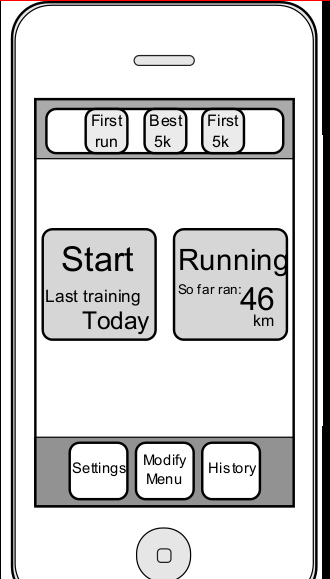
\includegraphics[width=0.5\textwidth]{Glowny2.jpg}
  \captionof{figure}{Ekran główny biegacza}
  \label{G2}
\end{minipage}
\begin{minipage}{0.5\textwidth}
Przyciski:\\
\begin{description}
  \item[Start] -- powinien prowadzić do ekranu wyboru sportów (rys. ~\ref{S1}). Tekst powinien odzwierciedlać stan treningu użytkownika -- jak długo już trenuje z aplikacją, szczególne osiągnięcia.
  \item[Settings] -- powinien prowadzić do ekranu opcji. Nie powinien mieć na sobie żadnego tekstu poza "Settings". Ekran opcji powinien zawierać różne opcje, w zależności od platformy i implementacji, pozwalające na dopasowanie działania aplikacji do oczekiwań użytkownika.
  \item[Main menu] -- napis na górnym pasku powinien zawierać powiadomienia o nowych dla użytkownika rzeczach (osiągnięciach, otrzymanych nagrodach). Mogą to być przyciski do bardziej szczegółowych opisów.
  \item[History] -- powinien pozwalać na przejście do ekranu, w którym użytkownik może zobaczyć poprzednie treningi z aplikacją i ich podsumowania.
  \item[Modify menu] -- po jego naciśnięciu użytkownik powinien mieć możliwosć modyfikacji ekranu głównego przez dodanie nowych przycisków -- p. dodatkowe przyciski, poniżej. Powinno odbywać się to w stylu zgodnym z platformą na jakiej aplikacjia jest uruchomiona.
  \item[Dodatkowe przyciski] -- powinny pojawiać się w miarę treningu użytkownika z aplikacją, np. jeśli dużo biega to powinien pojawić się tu przycisk "Running", taki sam jak w ekranie wyboru sportów (rys.~\ref{S1}, rys.~\ref{PR}). Ułatwi to użytkownikowi szybkie rozpoczynanie treningów, bez zbędnego kilkania.
\end{description}
\end{minipage}
\subsection{Sporty}
\subsubsection{Opis}
\noindent Podobnie jak w ekranie głównym, ekran ten powinien dopasowywać się do użytkownika. Tutaj powinno odbywać się to przez pojawianie się dodatkowego tekstu na przyciskach, opisującego stan treningu w danym trybie. Aplikacja powinna pozwalać na dodanie nowych trybów treningowych. Z tego ekranu powinno być możliwe przejście do każdego z dostępnych aktualnie trybów treningowych.
\subsubsection{Ekran}
\begin{minipage}{0.5\textwidth}
  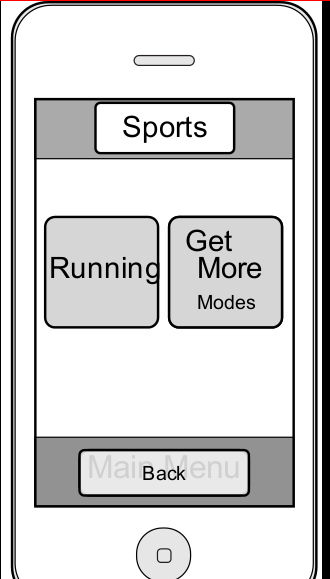
\includegraphics[width=0.5\textwidth]{Sports1.jpg}
  \captionof{figure}{Ekran start po pierwszym uruchomieniu}
  \label{S1}
  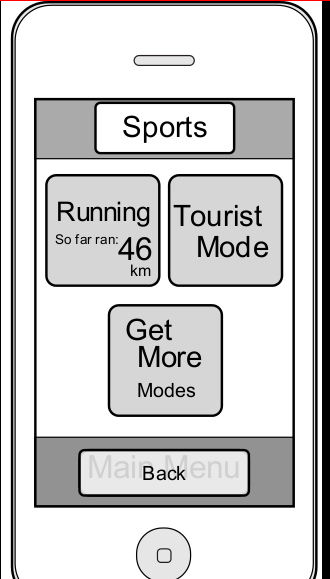
\includegraphics[width=0.5\textwidth]{Sports2.jpg}
  \captionof{figure}{Ekran start po dodaniu nowego trybu}
  \label{S2}
\end{minipage}
\begin{minipage}{0.5\textwidth}
Przyciski:\\
\begin{description}
  \item[Get more] -- powinien pozwalać na dodanie (np. pobranie ze sklepu, instalacja z wcześniej pobranej paczki lub wpisanie klucza) dodatkowego trybu treningowego.
  \item[Back] -- cofnięcię się do poprzedniego ekranu (w tym przypadku głównego).
  \item[Dodatkowe przyciski] -- dla każdego dostępnego trybu treningowego powinien być osobny przycisk (np. rys.~\ref{PR}), którego wygląd powinien odzwierciedlać postępy użytkownika w tym trybie.
\end{description}
\end{minipage}
\subsection{Running}
\subsubsection{Opis}
\noindent W podstawowj wersji, aplikacja ,,Iron Coach'' powinna zawierać przynajmniej moduł do biegania, którego makieta została tutaj opisana. Ekran ,,Plan a run'' pozwala na wybranie, w jakim trybie użytkownik chce biec. Dostępny powinien być przynajmniej tryb ,,Distance run''.
\subsubsection{Ekran}
\begin{minipage}{0.5\textwidth}
  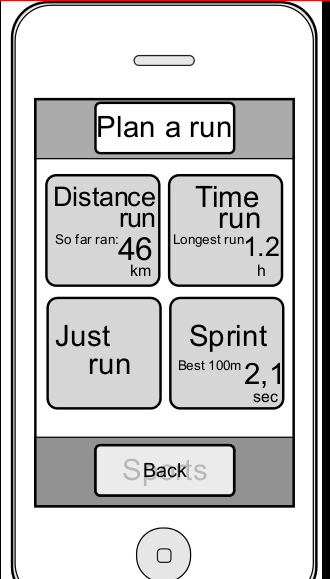
\includegraphics[width=0.5\textwidth]{PlanARun.jpg}
  \captionof{figure}{Ekran ,,Plan a run'' z czterema dostępnymi trybami}
  \label{PR}
\end{minipage}
\begin{minipage}{0.5\textwidth}
Przyciski:\\
\begin{description}
  \item[Back] -- powinien cofać do ekranu, z którego użytkownik przeszedł do obecnego.
  \item[Dodatkowe przyciski] -- każdy z nich powinien przenosić do innego z dostępnych trybów treningowych (np. rys.~\ref{DR}), a wygląd powinien odzwierciedlać postępy w tym trybie.
\end{description}
\end{minipage}
\subsection{Distance run}
\subsubsection{Opis}
\noindent Ekran ten ma pozwolić użytkownikowi na dopasowanie, na jaki dokładnie dystans i jaką trasą chce biec. Ma dawać użytkownikowi możliwość trenigu progresywnego, przez wybieranie stopniowo dłuższych tras.
\subsubsection{Ekran}
\begin{minipage}{0.5\textwidth}
  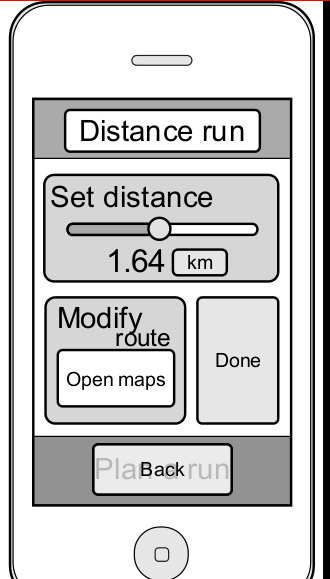
\includegraphics[width=0.5\textwidth]{DRun.jpg}
  \captionof{figure}{Ekran ,,Distance run'' z wybranym dystansem}
  \label{DR}
\end{minipage}
\begin{minipage}{0.5\textwidth}
Przyciski:\\
\begin{description}
  \item[Back] -- powinien cofać do ekranu, z którego użytkownik przeszedł do obecnego.
  \item[Done] -- powinien przenosić do ekranu potwierdzenia (rys.~\ref{RR}).
  \item[Set distance] -- powinien pozwalać na wybór długośći trasy. Wybór ten powinien być uwzględniony przy tworzeniu przykładowej trasy, jaka zostanie zaproponowana. Dodatkowe przebiegnięcie tego dystansu powinno być zasygnalizowane użytkownikowi.
  \item[Open maps] -- powinien przenosić do ekranu mapy (rys.~\ref{M}) i dopasowanie szczegółów trasy.
\end{description}
\end{minipage}
\subsubsection{Ostrzeżenia}
\noindent Może okazać się, że użytkownik wybierze bardzo długi lub krótki dystans (ogólnie lub w porównaniu z poprzednimi). Przed przejściem do kolejnego ekranu należy się upewnić, czy nie był to przypadek.
\subsection{Maps}
\subsubsection{Opis}
\noindent Tutaj użytkownik powinien mieć możliwość dopasowania szczegółów trasy, jaką chce pobiec. Kilka tras powinno być już zasugerowanych (na podstawie poprzednich, wybranego dystansu, często bieganych przez innych użytkowników, itd).
\subsubsection{Ekran}
\begin{minipage}{0.5\textwidth}
  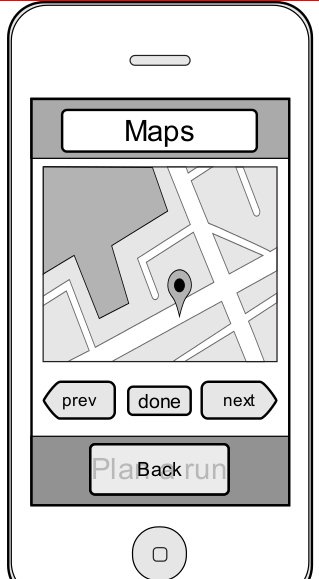
\includegraphics[width=0.5\textwidth]{Maps.jpg}
  \captionof{figure}{Ekran map}
  \label{M}
\end{minipage}
\begin{minipage}{0.5\textwidth}
Przyciski:\\
\begin{description}
  \item[Back] -- powinien cofać do ekranu, z którego użytkownik przeszedł do obecnego.
  \item[Strzałki] -- powinny pozwalać na wybór w kilku sugerowanych tras.
  \item[Done] -- powinien zatwierdzać wybór trasy.
  \item[Mapa] -- klikanie i przeciąganie trasy na mapie powinno modyfikować trasę. Ogólnie nawigacja mapą powinna być znana użytkownikowi z innych aplikacji (np Google Maps©).
\end{description}
\end{minipage}
\subsubsection{Ostrzeżenia}
\noindent Może okazać się, że nie można wyświetlić proponowanej trasy: może nie być pobrana, a użytkownik nie zezwolił na pobranie w tym momencie. Należy go o tym poinformować i nie wyświetlać tego ekranu. Może też się okazać, że wyłączony jest GPS i nie można ustalić pozycji użytkownika -- wówczas należy pozwolić użytkownikowi na własnoręczne wykreślenie trasy lub wybór z poprzednich. Może być i tak, że według danych aplikacji wybraną trasą nie można biec - np prowadzi przez rzekę bez mostu. O tym należy tylko poinformować użytkownika -- może okazać się, że wie o czymś, czego nie ma na mapie (lub potrafi dobrze pływać).
\subsection{Gotów do biegu}
\subsubsection{Opis}
\noindent Celem tego ekranu jest upewnienie się, że użytkownik wybrał już wszystkie opcje i chce rozpocząć bieg. 
\subsubsection{Ekran}
\begin{minipage}{0.5\textwidth}
  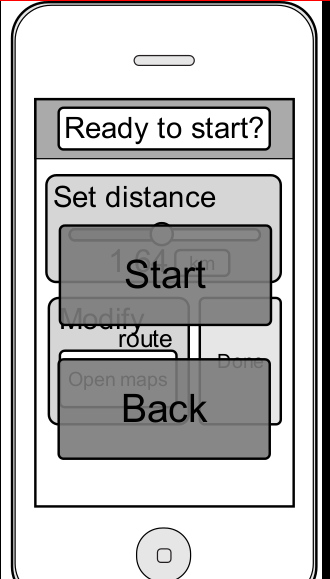
\includegraphics[width=0.5\textwidth]{Ready.jpg}
  \captionof{figure}{Potwierdzenie, że użytkownik chce rozpocząć bieg}
  \label{RR}
\end{minipage}
\begin{minipage}{0.5\textwidth}
Przyciski:\\
\begin{description}
  \item[Back] -- powinien cofać do ekranu, z którego użytkownik przeszedł do obecnego.
  \item[Start] -- powinien rozpoczynać bieg (przenosić do rys.~\ref{R}).
\end{description}
\end{minipage}
\subsection{Running}
\subsubsection{Opis}
\noindent Ekran śledzenia biegu -- obrazuje stan biegu: ile użytkownik już przebiegł, ile czasu mu to zajęło, jaką dalszą trasą powinien biec.
\subsubsection{Ekran}
\begin{minipage}{0.5\textwidth}
  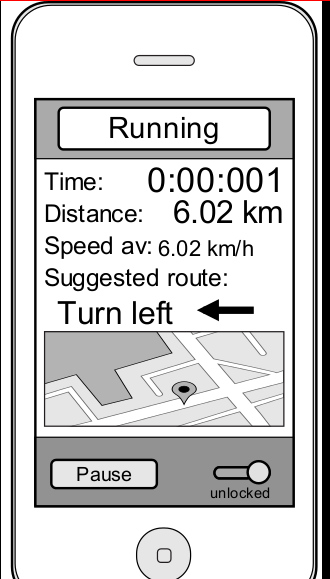
\includegraphics[width=0.5\textwidth]{Running.jpg}
  \captionof{figure}{Ekran biegu}
  \label{R}
\end{minipage}
\begin{minipage}{0.5\textwidth}
Przyciski:\\
\begin{description}
  \item[Lock] -- pozwala zablokować ekran, by nie dało się nic kliknąć: sposób odblokowania właściwy do platformy z jakiej korzysta użytkownik, na iOS-ie może to być przycisk ,,unlock'', który trzeba przesunąć.
  \item[Pause] -- powinien pauzować bieg (rys.~\ref{RP}).
\end{description}
\end{minipage}
\subsection{Pauza}
\subsubsection{Opis}
\noindent Ekran ten powinien być włączony, gdy użytkownik nie biegnie -- może się włączać automatycznie. Przestój może oznaczać, że użytkownik się zmęczył i chce przerwać bieg, rozmawia ze znajomym lub próbuje się zorientować jak biec dalej, bo trasa jaką planował jest zablokowana.
\subsubsection{Ekran}
\begin{minipage}{0.5\textwidth}
  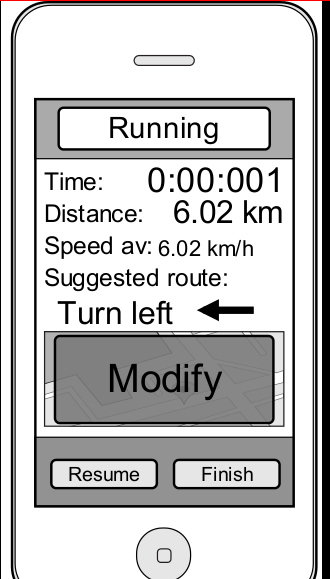
\includegraphics[width=0.5\textwidth]{RPaused.jpg}
  \captionof{figure}{Ekran pauzy}
  \label{RP}
\end{minipage}
\begin{minipage}{0.5\textwidth}
Przyciski:\\
\begin{description}
  \item[Resume] -- pozwala na kontynuację biegu.
  \item[Finish] -- użytkownik chce zakończyć aktualny bieg (rys.~\ref{RS}).
  \item[Modify] -- trasa przestała odpowiadać użytkownikowi, chce ją zmienić. Przenosi do ekranu ,,Maps'' (rys.~\ref{M}).
\end{description}
\end{minipage}
\subsection{Run Summary}
\subsubsection{Opis}
\noindent Ekran ten jest opisem zakończonego biegu: trasy, czasu i innych zapamiętanych szczegółów.
\subsubsection{Ekran}
\begin{minipage}{0.5\textwidth}
  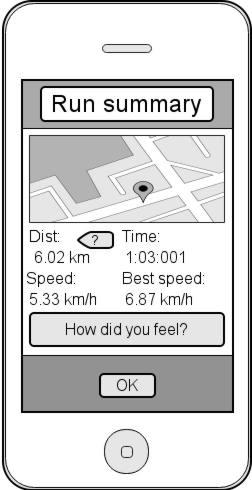
\includegraphics[width=0.5\textwidth]{RSummary.jpg}
  \captionof{figure}{Ekran podsumowania}
  \label{RS}
\end{minipage}
\begin{minipage}{0.5\textwidth}
Przyciski:\\
\begin{description}
  \item[OK] -- pozwala na przejście dalej: jego zachowanie powinno być różne w zależności skąd użytkownik przeszedł do tego ekranu. Jeśli poprzednim ekranem był ekran biegu, to ten przycisk powinien przenosić do ekranu głównego. Jeśli był to ekran historii, to ten przycisk powinien do niego cofać.
  \item[?] -- pozwala na poprawę szczegółów: być może trasa została źle wyznaczona lub dystans czy czas były inne (błąd pomiaru).
  \item[How did you feel?] -- powinien pozwalać użytkownikowi na zapisanie dodatkowej obserwacji związanej z tym biegiem: jak się po nim czuł (rys.~\ref{HF}). Pozwoli to na ocenę, jak użytkownik lubi biegać.
\end{description}
\end{minipage}
\subsubsection{Ostrzezenia}
\noindent Ponieważ w tym ekranie użytkownik ma możliwość zmiany szczegółów, to przed wyjściem z niego należy się upewnić, że użytkownik chce ewentualne zmiany zapisać.
\subsection{How did you feel?}
\subsubsection{Opis}
\noindent Ekran ten pozwala użytkownikowi określić, jak się czuje po biegu.
\subsubsection{Ekran}
\begin{minipage}{0.5\textwidth}
  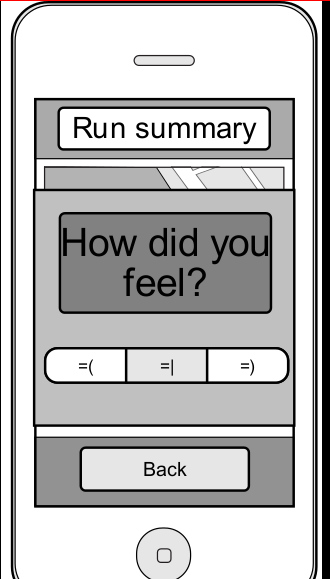
\includegraphics[width=0.5\textwidth]{Feelings.jpg}
  \captionof{figure}{Ekran oceny samopoczucia}
  \label{HF}
\end{minipage}
\begin{minipage}{0.5\textwidth}
Przyciski:\\
\begin{description}
  \item[=(] -- symbolizuje złe samopoczucie.
  \item[=|] -- symbolizuje neutralne samopoczucie.
  \item[=)] -- symbolizuje dobre samopoczucie.
\end{description}
\end{minipage}
\end{document}
